\chapter{Das Hadoop Ecosystem}
Im Laufe der Jahre hat sich um den Kern von Hadoop ein reichhaltiges Ökosystem an weiteren Projekten gebildet (das Hadoop Ecosystem). Diese erweitern die Funktionalitäten des Kerns, oder ersetzen gar ganze Komponenten durch alternative Implementierungen. Hadoop ist so modular konzipiert, dass dies problemlos möglich ist.  \\
Das Ecosystem lässt sich grob in vier Kategorien aufteilen: Datenspeicherung, Verwaltung~/~Konfiguration, Datentransfer und Datenverarbeitung (\textit{vgl. Abb. }\ref{fig:ecosys}). Die Komponenten in \textit{Abb. }\ref{fig:ecosys} sollen in den nächsten Abschnitten kurz angerissen werden, um dann in den jeweiligen Kapiteln tiefergehend auf die Nutzung einiger ausgesuchter Komponenten einzugehen.

\begin{figure}[ht]
    \centering
    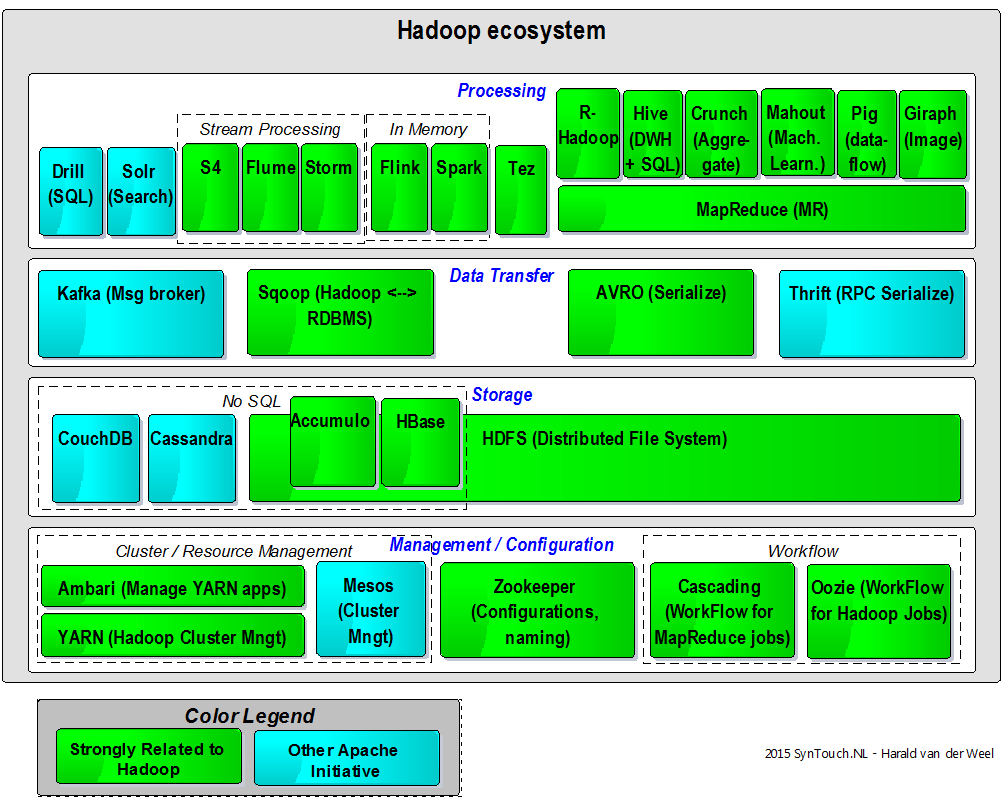
\includegraphics[width=\textwidth]{Hadoop_ecosystem_overview}
    \caption[Komponenten des Hadoop Ecosystems]{Komponenten des Hadoop Ecosystems\parencite{van_der_weel_hadoop_2015}}
    \label{fig:ecosys}
\end{figure}

\section{Datenhaltung}
\subsection*{HDFS}
Hadoops primäres Dateisystem, siehe 
\subsection*{HBase}

\section{Cluster-Verwaltung / -Konfiguration}
\subsection*{YARN}
\subsection*{Oozie}
\subsection*{ZooKeper}
\subsection*{Ambari}

\section{Datentransfer}
\subsection*{Sqoop}
\subsection*{Kafka}
\subsection*{AVRO}

\section{Datenverarbeitung}
\subsection*{MapReduce}
\subsection*{Tez}
\subsection*{Pig}
\subsection*{Hive}
\subsection*{Flume}
\subsection*{Mahout}
\subsection*{Spark}
\subsection*{Solr}
